\documentclass[letterpaper]{article}

%% Language and font encodings
\usepackage[english]{babel}
\usepackage[utf8x]{inputenc}
\usepackage[T1]{fontenc}

%% Sets page size and margins
\usepackage[letterpaper,top=2.5cm,bottom=2cm,left=2cm,right=2cm,marginparwidth=1.75cm]{geometry}

%% Useful packages
\usepackage{amsmath}
\usepackage{amssymb}
\usepackage{amsfonts}
\usepackage{graphicx}
\usepackage[colorinlistoftodos]{todonotes}
\usepackage[colorlinks=true, allcolors=blue]{hyperref}
\usepackage{listings}
\usepackage{multicol}
\usepackage{float}

\usepackage{bm}
\date{\today}

\title{CSC411 Assignment 1}
\author{Yue Guo}
\begin{document}
\maketitle

%\centering
%  \includegraphics[width=0.5\textwidth]{1.3.2/1_3_2_k50.png}
%  \caption{k-NN Regression of $x \in [0, 11]$ with $k$ = 50.}
%\end{figure}

\section{Learning basics of regression in Python }

\subsection{Describe and summarize the data}
Dimension: 13\\
Target: price\\
Data points: for each feature, we have 506 data points

\subsection{visualization}
\subsection{}
\begin{figure}[H]
\centering
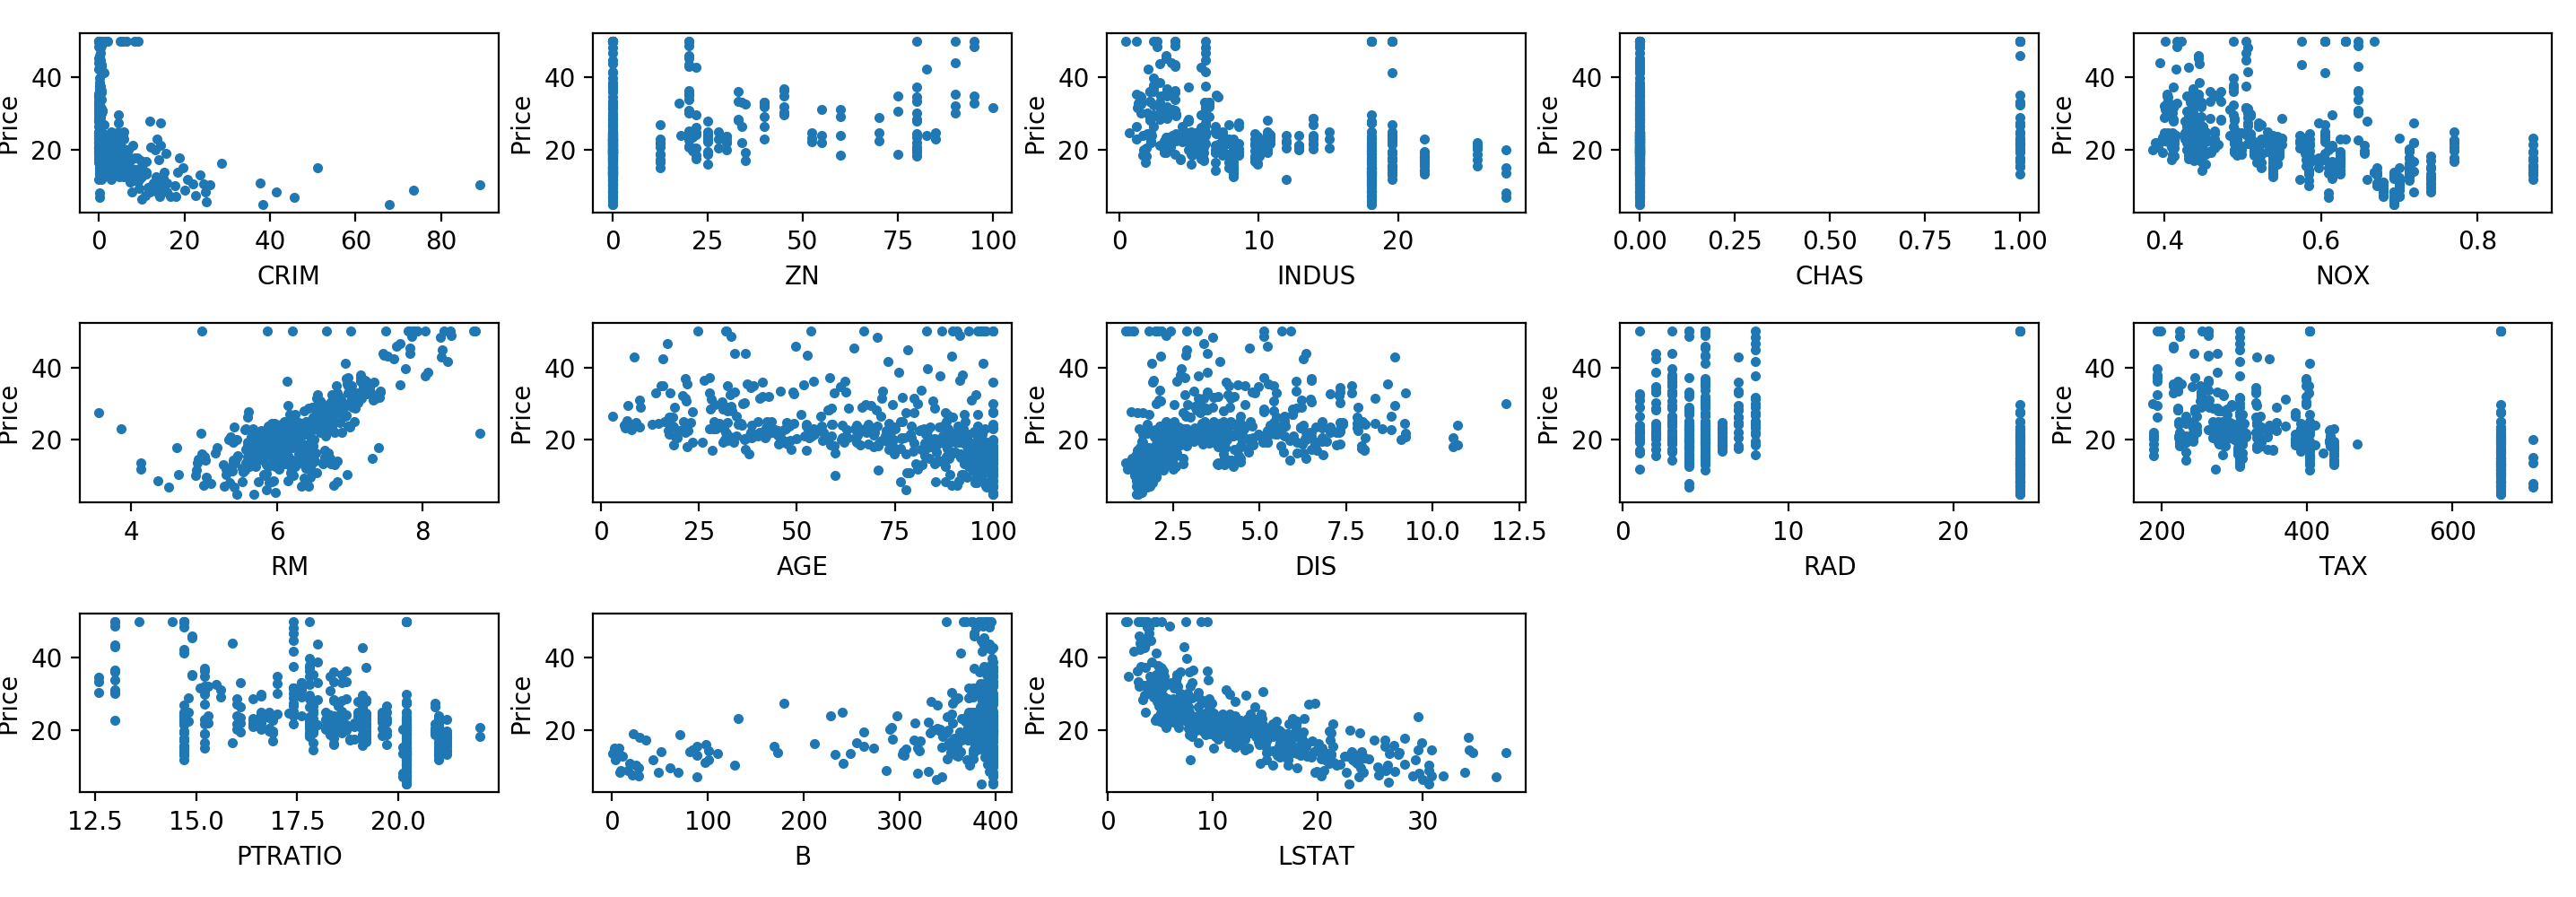
\includegraphics[width=1\textwidth]{Figure_1.png}
\caption{\label{fig:q1}}
\end{figure}


\subsubsection{Feature weights}


Weights of each feature: \\
\begin{center}
\begin{tabular}{ |c|c| } 
 \hline
CRIM  & 39.3306546864 \\
ZN & -0.105570660997\\
INDUS  & 0.033569463917\\
CHAS & 0.0501338462503\\
NOX & 2.44159672082\\
RM  &-18.9563291605\\
AGE  & 3.65717113479\\
DIS & 0.00193877592741\\
RAD  & -1.46699325228\\
TAX & 0.349594800713\\
PTRATIO  &-0.0145786907583\\
B & -0.959592750851\\
LSTAT & 0.008452561222\\
 \hline
\end{tabular}
\end{center}
INDUS matches my expectation. The more business we have, the more prosperous an area is, therefore more expensive housing.

\subsubsection{MSE of my model}
19.0490487755

\subsubsection{Two more error measurement}

normal error = 313.546384855\\
mean square root= 0.281596677525\\
I suggest these two error measurements because they do not square the differences.


\subsubsection{Most significant feature}
Based on my results, the most significant feature is RM and CRIM. It has larger weight value among all features.
 



%%%%%%%%Q 2%%%%%%%%%%%
\section{Locally weighted regression}

\subsection{weighted least square problem and analytic solution proof}
Since the matrix A is diagonal and $\hat{y} =A^T x$ and $L(w) = \frac{1}{2} \Sigma a^{(i)}(y^{(i)} - W^T x^{(i)} )^{2} + \frac{\lambda}{2} \lVert W \rVert ^{2}$ \\
$ L(w) = \frac{1}{2} A [(y - W^T x)(y - W^T x)] + \frac{\lambda}{2} \lVert W \rVert ^{2}$\\
$ L(w) = \frac{1}{2} A (y^T y + W^T X^T XW -2W^T  X^T y) +\frac{\lambda}{2}  \lVert W \rVert ^{2}$\\
$ \frac{\partial}{\partial{w}} =\frac{1}{2} \times 2 A[X^T X W^{*} - X^T y] + \lambda \lVert W \rVert = 0$\\
$A X^T X W^{*} - X^T Ay + \lambda W^{*} = 0 $\\
$(A X^T X + \lambda)W^{*} = X^T Ay  $\\
$W^{*} = X^T Ay (A X^T X + \lambda I)^{-1} $


\subsection{}
x is Tau, y is losses
\begin{figure}[H]
\centering
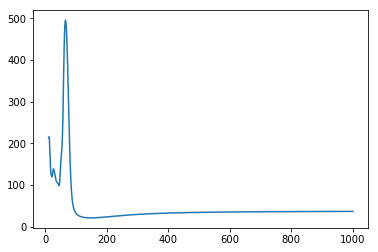
\includegraphics[width=0.5\textwidth]{q2_final.png}
\caption{\label{fig:q2}}
\end{figure}

\subsection{}
The algorithm produces results or weights of each feature with a large variance if $\tau$ -> 0,  and
 variance -> constant if $\tau $-> $\inf$
 
 %%%%%%%%%%%% Q3%%%%%%%%%%%%%
\section{Mini-batch}
\subsection{Proof of expected value of mini batches}
$RHS = \frac{1}{n} \Sigma_{i=1}^{n}a_{i}$ is the average of all samples in the data set\\
LHS: $ \frac{1}{m}  \Sigma_{i=1}^{m} a_{i} $ is the average of each random batch. Since each batch is drown randomly from the dataset, the m elements each have $ \frac{1}{n}$ chance to be drawn. The probability of the batch is $ \frac{m}{n}$. $E(\frac{1}{m} \Sigma  a_{i}) = \frac{m}{n} \times  \frac{1}{m} \Sigma  a_{i} = \frac{1}{n} \Sigma_{i=1}^{n} a_{i} $ \\
QED

\subsection{Proof of gradients}
From the result of part 1,  substitute $l$ into $a_{i}$\\
$E[ \frac{1}{m} \Sigma l(x ,y,  \theta)  ] = \frac{1}{n} \Sigma l(x ,y, \theta) $\\
$E[L(x, y, \theta)] = L(x ,y, \theta)$\\
apply gradient, we have \\
$\nabla E[L(x, y, \theta)] =\nabla L(x ,y, \theta) =  \frac{1}{n} \Sigma_{i=1}^{n} \nabla l $\\
$\nabla \frac{1}{n} \Sigma_{i=1}^{n} l  = \nabla E(\frac{1}{m} \Sigma  a_{i}) $ \\
$E[ \nabla L(x, y, \theta)] = \nabla L(x, y, \theta) $

\subsection{Importance of this result}
This implies that k random batches of data can approximate the gradient of the complete dataset.

\subsection{Gradient}
\subsubsection{Analytic solution}
$\nabla L = 2X^TXw - 2X^Ty$
\subsubsection{}
see q3.py

\subsection{Error measurements}
square metric = 79165708.6263 \\
cosine similarity =  0.999998432222\\
I suggest cosine similarity because square distance takes the difference to the power of 2, which punishes certain cases more. 

 
\subsection{plot}
X axis is weights, y axis is log of M

this is the graph if we average all the weights
\begin{figure}[H]
\centering
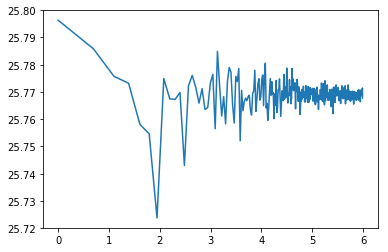
\includegraphics[width=0.5\textwidth]{q3_final.png}
\caption{\label{}}
\end{figure}

This is the graph if we average each $w_{j}$
X axis is weights, y axis is log of M

\begin{figure}[H]
\centering
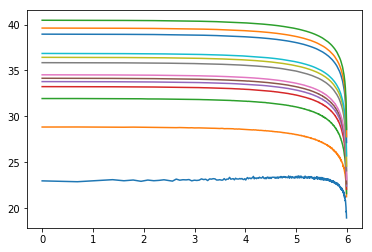
\includegraphics[width=0.5\textwidth]{q3_f2.png}
\caption{\label{fig:q3}}
\end{figure}





% \section{Some examples to get started}

% \subsection{How to add Comments}

% Comments can be added to your project by clicking on the comment icon in the toolbar above. % * <john.hammersley@gmail.com> 2014-09-03T09:54:16.211Z:
% %
% % Here's an example comment!
% %
% To reply to a comment, simply click the reply button in the lower right corner of the comment, and you can close them when you're done.

% \subsection{How to include Figures}

% First you have to upload the image file from your computer using the upload link the project menu. Then use the includegraphics command to include it in your document. Use the figure environment and the caption command to add a number and a caption to your figure. See the code for Figure \ref{fig:frog} in this section for an example.

% \begin{figure}
% \centering
% \includegraphics[width=0.3\textwidth]{frog.jpg}
% \caption{\label{fig:frog}This frog was uploaded via the project menu.}
% \end{figure}

% \subsection{How to add Tables}

% Use the table and tabular commands for basic tables --- see Table~\ref{tab:widgets}, for example. 


% \subsection{How to write Mathematics}

% \LaTeX{} is great at typesetting mathematics. Let $X_1, X_2, \ldots, X_n$ be a sequence of independent and identically distributed random variables with $\text{E}[X_i] = \mu$ and $\text{Var}[X_i] = \sigma^2 < \infty$, and let
% \[S_n = \frac{X_1 + X_2 + \cdots + X_n}{n}
%       = \frac{1}{n}\sum_{i}^{n} X_i\]
% denote their mean. Then as $n$ approaches infinity, the random variables $\sqrt{n}(S_n - \mu)$ converge in distribution to a normal $\mathcal{N}(0, \sigma^2)$.


% \subsection{How to create Sections and Subsections}

% Use section and subsections to organize your document. Simply use the section and subsection buttons in the toolbar to create them, and we'll handle all the formatting and numbering automatically.

% \subsection{How to add Lists}

% You can make lists with automatic numbering \dots

% \begin{enumerate}
% \item Like this,
% \item and like this.
% \end{enumerate}
% \dots or bullet points \dots
% \begin{itemize}
% \item Like this,
% \item and like this.
% \end{itemize}

% \subsection{How to add Citations and a References List}

% You can upload a \verb|.bib| file containing your BibTeX entries, created with JabRef; or import your \href{https://www.overleaf.com/blog/184}{Mendeley}, CiteULike or Zotero library as a \verb|.bib| file. You can then cite entries from it, like this: \cite{greenwade93}. Just remember to specify a bibliography style, as well as the filename of the \verb|.bib|.

% You can find a \href{https://www.overleaf.com/help/97-how-to-include-a-bibliography-using-bibtex}{video tutorial here} to learn more about BibTeX.

% We hope you find Overleaf useful, and please let us know if you have any feedback using the help menu above --- or use the contact form at \url{https://www.overleaf.com/contact}!

% \bibliographystyle{alpha}
% \bibliography{sample}

\end{document}